\chapter{Evaluation and Analysis}

In the first part of this section we briefly depict the nature of the data set used for evaluation of the models and discuss some specifics of the implementation. In the next part we present the results of our analysis.

\section{Data Set}

For the analysis we used data from the online system for practicing geography\footnote{\url{http://www.slepemapy.cz}}~\cite{Papousek2014}. The data set contains more than 10~million answers from thousands of unique users~\cite{Papousek2015}. The data were filtered to contain only students with at least 50 answers and usually divided into 5 data sets, each containing at least 30 thousand answers. The answers of students who registered before the oldest question in the data set was answered were removed since it could temper with the results (considering we are interested primarily in models based on timing information).

\section{Toolchain}

The models were implemented in Python programming language. Experiments were performed in the Jupyter Notebook interactive environment\footnote{Jupyter Notebook is an open sourced web application for interactive computing, see~\url{https://jupyter.org/}}. Here is a list of the used libraries and modules:

\begin{itemize}
  \item SciPy, NumPy, Pandas
  \item Scikit-Learn
  \item Matplotlib
  \item NetworkX
\end{itemize}

\section{Response Time}

The response time of student to a question indicates how much well the item is learned. If the student answered quickly, almost automatically, it is very likely they either know the place very well or don't at all, depending on the correctness of their answer. On the other hand when the response is longer, the student is probably familiar with the item and might even recall the correct answer.

The Figure~\ref{fig-response-time} demonstrates the relationship between students' response time and the probability of recall. If the student's answer was suspiciously fast (response time is lower than 800 milliseconds), it usually means they are guessing. If the response time is between 1500 and 2000 milliseconds, it may indicate the student knows the correct answer.

Note that some places are bigger on the map then other, i.e. a question requiring the student to choose Russia on the map has generally lower response time than a question requiring to choose Andorra.

\begin{figure}[htbp]
  \centering
  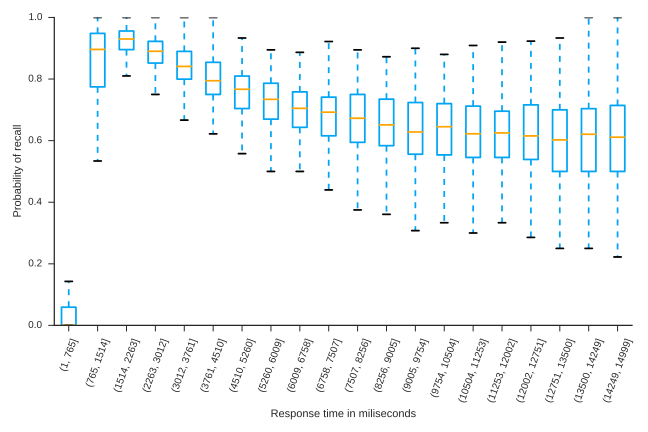
\includegraphics[width=\textwidth]{img/response-time}
  \caption{Relation between students' response time and probability of recall. Each box represents probabilities from all countries that belong in the relevant interval of response times.}
  \label{fig-response-time}
\end{figure}

\section{Memory Decay}

In this chapter we evaluate and analyze several models with the focus on memory decay and forgetting. Since we use abbreviations for the models, here is a list of all evaluated models as they occur in our experiments:

\begin{itemize}
  \item \textbf{PFA} -- this is the original performance factor analysis which we described in chapter~\ref{pfa}. Our implementation, however doesn't consider multiple knowledge components as there is only one.
  \item \textbf{PFA/E} -- a version of the original PFA model with some aspects of Elo model we depicted in chapter~\ref{pfae}.
  \item \textbf{PFA/E/T} -- an extended version of the PFA/E model which adapts the idea of a time effect function. We presented the model in chapter~\ref{pfaet}. In our analysis we examined several time effect functions.
  \item \textbf{PFA/G} -- another version of the original PFA model with a decay factor, the characteristics of the model were outlined in chapter~\ref{pfag}. The implementation doesn't consider multiple knowledge components.
  \item \textbf{PFA/G/T} -- our version of the PFA/G model which uses a time effect function instead of a decay factor. The differences were stated in chapter~\ref{pfagt}.
\end{itemize}

Note that in some analyses we also use the Elo model briefly described in chapter~\ref{elo} for the estimation of prior knowledge.

\subsection{Parameters}

Standard PFA model has 3 parameters, the initial difficulty of an item $\beta$, weight of each success $\gamma$ and failure $\delta$. In cases where we use Elo model for prior knowledge estimation, we can replace the parameter $\beta$ with $\theta_s - b_c$ which leaves us with only 2 parameters we need to estimate. Nevertheless, a time effect function has to be chosen as well for the PFA/E/T and PFA/G/T models.

\subsection*{Time Effect Functions}

In chapter~\ref{memory} we mentioned that forgetting usually respects the power law, which is often true in cases where the students have no prior knowledge of the practiced material. We tested several simple analytical function:

\begin{itemize}
  \item $f(t) = a - c \cdot \log(t)$
  \item $f(t) = a \cdot e^{c t}$
  \item $f(t) = a / t^c$
\end{itemize}

Figures of each of these time effect functions with logarithmically scaled $x$-axis can be seen on the figure~\ref{fig-time-effect-functions}. As all functions have only the two parameters $a$ and $c$, we optimized them with the greedy search algorithm detailed in chapter~\ref{greedy-search}.

\begin{figure}[htbp]
  \centering
  \includegraphics[width=\textwidth]{img/time-effect-functions}
  \caption{Candidates of time effect functions we inspected and evaluated in our analysis. Note that the $x$-axis is log scaled.}
  \label{fig-time-effect-functions}
\end{figure}

The used data set contains genuinely very different students with distinct prior knowledge, some students are still in school and practice geography in classes, other students already finished school and want to revive their forgotten knowledge (this is further analyzed in chapter~\ref{further-analysis}). There are also tremendous differences between continents, regions and types of places, all of which vary in the easiness of learning, some are harder to retain and are forgotten faster. These attributes make it very different from standard models that try to capture the students with fixed age or no prior knowledge of the learned material.

Since our goal is to model the forgetting of students who use the system for practicing geography slepemapy.cz, probably the most accurate and best calibrated model can be achieved by learning the time effect function from the data set by using the adjusted gradient descent described in chapter~\ref{gradient-descent}.

Because we want to approximate the exact shape of time effect function, we need to define a staircase function with fixed intervals $\boldsymbol{I}$. In each interval $(I_k, I_{k+1}\rangle$, we preserve a learned value $a_k$ which represents an increase in memory activation. The formal definition of the staircase function $f(t)$ is formalized in Equation~\ref{eq-staircase}.

\begin{equation} \label{eq-staircase}
  f(t) = \begin{cases}
            a_1, & \text{if } I_0 < t \leq I_1 \\
            a_2, & \text{if } I_1 < t \leq I_2 \\
                 & \hspace{1em} \dots \\
            a_n, & \text{if } I_{n-1} < t \leq I_n
         \end{cases}
\end{equation}

Applying simple linear algebra, we can further modify the staircase function so that the memory activation between two points is a linear function, which makes a better approximation of the learned values:

\begin{equation} \label{eq-staircase-2}
  f(t) = \begin{cases}
            a_1, & \text{if } I_0 < t \leq I_1 \\
            (t - a_1) \frac{I_2 - I_1}{a_2 - a_1} + I_1, & \text{if } I_1 < t \leq I_2 \\
            \hspace{9em} \dots \\
            (t - a_{n-1}) \frac{I_n - I_{n-1}}{a_n - a_{n-1}} + I_{n-1}, & \text{if } I_{n-1} < t \leq I_n     
         \end{cases}
\end{equation}

Note that $I_0$ is in our case always equal to $0$ and $I_n$ to infinity (in which case the memory activation in the interval is equal to $a_n$).

In our experiments we divided the vector $\boldsymbol{I}$ in 10 intervals, we chose the following values: $(0s, 60s\rangle$,$(60s, 90s\rangle$, $(90s, 2.5m\rangle$, $(2.5m, 5m\rangle$, $(5m, 10m\rangle$, $(10m, 30m\rangle$, $(30m, 3h\rangle$, $(3h, 24h\rangle$, $(24h, 5d\rangle$, $(5d, \infty)$. The staircase function obtained using gradient descent for parameter optimization is illustrated in Figure~\ref{learned-time-effect-function}. Note that $\gamma = 1.814 \pm 0.276$ and $\delta = 0.827 \pm 0.095$.

\begin{figure}[htbp]
  \centering
  \includegraphics[width=\textwidth]{img/learned-time-effect-function}
  \caption{Time effect function as learned from the data with standard deviations. Each point represents average of 10 independent data sets containing answers of users who used the system continuously at least for one week and answered more than 100 answers.}
  \label{learned-time-effect-function}
\end{figure}

\subsection*{Calibration}

\subsection{Evaluation}
\label{evaluation}

\section{Further Analysis}
\label{further-analysis}
